{\begin{minipage}[b]{0.33\textwidth}
\raggedright
{\large 66}
\end{minipage}%
\begin{minipage}[b]{0.33\textwidth}
\centering{\textbf{К В А  Н Т} $\cdot$ \textsf{2 0 1 5 \slash \textnumero 5 - 6}}
\end{minipage}%

\begin{multicols}{2}
\fontsize{10}{10}\selectfont
\textit{Дмитрий Татаркин (Саранск, Мордовия),} \par
\textit{Иван Утешев (Саранск, Мордовия).} \par
Минимальное количество баллов, необходимое для получения золотой медали, составило 42,2 балла, для получения
серебряной медали – 33,0 баллов. Вот как выступила наша команда:\\\\
\fontsize{9.5}{12}\selectfont
\begin{tabular}{l c c c c c c c}
&Т1&Т2&Т3&Э1&Э2&Сумма&Медаль\\
&&&&&&баллов&\\
А.Красников&9,8&9,6&9,8&9,4&8,6&47,2& золотая\\
К.Воронин&9,3&8,4&9,4&8,5&6,6&42,2&золотая\\
Г.Корепанов&8,7&7,4&8,3&9,7&9,1&43,2&золотая\\
Д.Татаркин&9,3&8,9&6,3&9,7&8,9&43,1&золотая\\
И.Утешев&9,9&8,6&8,4&8,5&6,5&41,9&серебряная\\
\end{tabular}\\\par
\fontsize{10}{10}\selectfont
Ниже приводятся условия задач теоретического тура олимпиады.\\\\
\textbf{\centerline{\large{ТЕОРЕТИЧЕСКИЙ ТУР}}}\\\par

\textbf{Задача 1. Частицы от Солнца} (10 баллов)\par
 Фотоны, излучаемые с поверхности Солнца, и нейтрино из его ядра несут нам информацию о температурах Солнца, также могут подтвердить, что Солнце светит благодаря ядерным реакциям.\par
Во всех пунктах этой задачи примите массу Солнца $M_\odot$ = 2,00 $\cdot 10^{30}$ кг,его радиус $R_\odot$ = 7,00 $\cdot 10^8$  м, его мощность (энергия, излученная в единицу времени) $L_\odot$ = 3,85 $\cdot 10^{26}$  Вт и расстояние от Земли до Солнца $d_\odot$ = 1,50 $\cdot 10^{11}$ м.\par
\textit{Примечание:}\\
$$\int_{}^{}xe^{ax}dx = (\frac{x}{a}-\frac{1}{a^2})e^{ax}+const$$
$$\int_{}^{}x^2e^{ax}dx = (\frac{x^2}{a}-\frac{2x}{a^2}+\frac{2}{a^3})e^{ax}+const$$
$$\int_{}^{}x^3e^{ax}dx = (\frac{x^3}{a}-\frac{3x^2}{a^2}+\frac{6x}{a^3}-\frac{6}{a^4})e^{ax}+const$$\par

\textbf{Часть A. Излучение Солнца}\par
\textbf{A1.}
 Полагая, что Солнце излучает как абсолютно черное
тело, вычислите температуру $T_p$ поверхности Солнца.
(0,3 б.)\\\par
Спектр солнечного излучения может быть хорошо аппроксимирован распределением Вина. Соответственно, солнечная энергия, приходящая в единицу времени в единичном
диапазоне частот на некоторую площадку на Земле, зависит
от частоты так:\par
$$u(v)=A\frac{R^2_\odot}{d^2_\odot}\frac{2\pi h}{c^2}v^3exp(-\frac{hv}{k_{b}T_{p}}),$$\\
где $v$ - частота излучения, \textit{A} - площадь поверхности этой
площадки, нормальной к направлению падающего излучения, $k_{b}$ - постоянная Больцмана.\par
Рассмотрим солнечный элемент, который представляет
собой тонкий диск из полупроводникового материала площадью \textit{A}. Солнечный элемент расположен перпендикулярно
направлению падения солнечных лучей.\\\par
\textbf{A2.}
Используя приближение Вина, выразите полную мощность солнечного излучения \textit{P}, падающего на поверхность
солнечного элемента, через \textit{A} $, R_\odot$ , $d_\odot$ , $T_p$ и фундаментальные константы $с$ , $h$ , $k_b$ . (0,3 б.)\par
\textbf{A3.}
 Как зависит от частоты число фотонов $n_\gamma (v)$, падающих в единицу времени в единичном диапазоне частот на\\
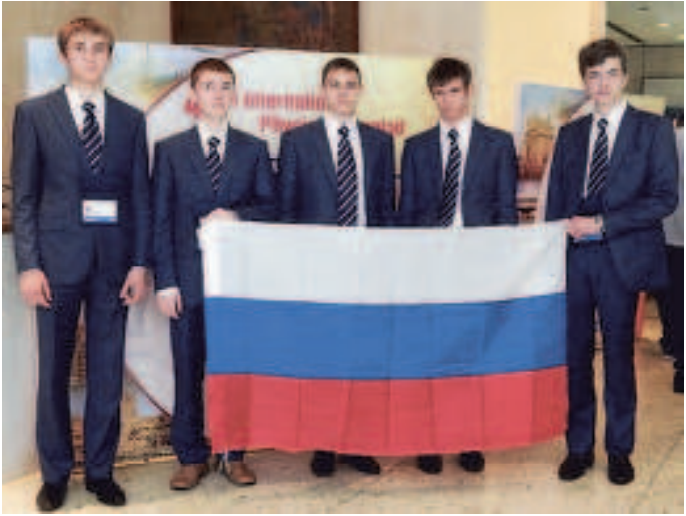
\includegraphics[height=2.9in]{image.png} \\
\fontsize{10}{11}\selectfont
\textit{Национальная сборная России. Слева направо: Д.Татаркин, И.Утешев, Г.Корепанов, А.Красников, К.Воронин}\\\\
поверхность солнечного элемента? Выразите ответ через \textit{A} , $R_\odot$ , $d_\odot$ , $T_p$ , $v$ и фундаментальные константы $c$ , $h$ , $k_b$.
(0,2 б.)\par
У полупроводника, из которого изготовлен солнечный
элемент, ширина запрещенной зоны $E_z$. Используйте следующую модель. Каждый фотон с энергией $E \geq E_z$
 позволяет электрону преодолеть запрещенную зону. Возбужденный
электрон может преобразовать в полезную энергию только
$E_z$, остальная часть энергии рассеивается в виде тепла (не
может быть преобразована в полезную).\par

 \textbf{A4.} Считайте, что $x_z$ = $hv_z/(k_bT_p$ , где $E_z$ = $hv_z)$. Выразите
полезную мощность солнечного элемента $P_{pol}$ через $x_z
,$ \textit{A} , $R_\odot$ , $d_\odot$ , $T_p$ и фундаментальные константы $c$ , $h$ , $k_b$. (1 б.)\par
 \textbf{A5.} Выразите КПД солнечного элемента $\eta$ через $x_z$.(0,2 б.)\par
 \textbf{A6.} Нарисуйте качественный график зависимости $\eta$ от $x_z$
. Явно укажите значения $\eta$ при $x_z = 0$ и $x_z \to \infty$. Чему
равен угловой коэффициент касательной к графику $\eta(x_z)$
при $x_z$ = $0$ и $x_z \to \infty?$ (1 б.)\par
 \textbf{A7.} Пусть $x_0$ – это такое значение $x_z$
, при котором $\eta$
максимален. Получите кубическое уравнение, для которого
$x_0$
 будет решением. Оцените численное значение $x_0$
 с
точностью ±0,25 . Рассчитайте также $\eta(x_0)$.(1 б.)\par
 \textbf{A8.}Ширина запрещенной зоны чистого кремния
$E_z = 1,11$ эВ. Рассчитайте КПД кремниевого солнечного
элемента $\eta_{Si}$ , используя это значение. (0,2 б.)\\\par
В конце XIX века Кельвин и Гельмгольц для объяснения
излучения Солнца предложили такую гипотезу. Они постулировали, что вначале Солнце было очень большим облаком
материи массой $M_\odot$ с пренебрежимо малой плотностью.
Затем Солнце постоянно сжималось. Таким образом, Солнце могло бы светить, постоянно теряя гравитационную
потенциальную энергию из-за своего медленного сжатия.\\\par
\textbf{A9.} Предположим, что плотность вещества внутри Солнца
всюду одинакова. Найдите полную гравитационную потенциальную энергию Солнца $\omega$ , которой оно обладает в наши
дни. Выразите ее через $G$ , $M_\odot$ и $R_\odot$. (0,3 б.)\par
\textbf{A10.} Считая, что мощность излучения Солнца оставалась
постоянной на протяжении всего времени, оцените максимально возможное время $\tau$ (в годах), на протяжении
которого Солнце могло светить согласно гипотезе Кельвина
и Гельмгольца. (0,5 б.)
\end{multicols}

